
\begin{figure}
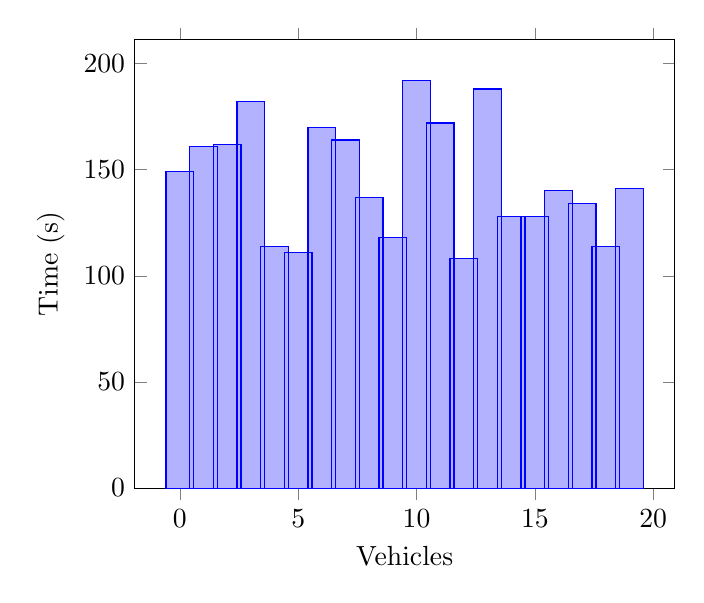
\begin{tikzpicture}
\begin{axis}[
legend style={anchor=west},
xlabel=Vehicles,
ylabel=Time (s),
ymin=0,
ybar,
]
\addplot coordinates {
(0, 149)
(1, 161)
(2, 162)
(3, 182)
(4, 114)
(5, 111)
(6, 170)
(7, 164)
(8, 137)
(9, 118)
(10, 192)
(11, 172)
(12, 108)
(13, 188)
(14, 128)
(15, 128)
(16, 140)
(17, 134)
(18, 114)
(19, 141)
};

\end{axis}
\end{tikzpicture}
\label{tik:100:3_V, 3_V.-60, 4_S, 5_S, 5_S.-30, 7_S, 7_S.-25, 11_S, 11_S.-50, 13_S, 15_N, 17_S, 17_S.-60, 19_V}
\caption{100 percent diving with GSC on route $3_V, 3_V.-60, 4_S, 5_S, 5_S.-30, 7_S, 7_S.-25, 11_S, 11_S.-50, 13_S, 15_N, 17_S, 17_S.-60, 19_V$}
\end{figure}
